\documentclass{standalone}
\usepackage{tikz}
\usetikzlibrary{patterns, positioning}

\begin{document}
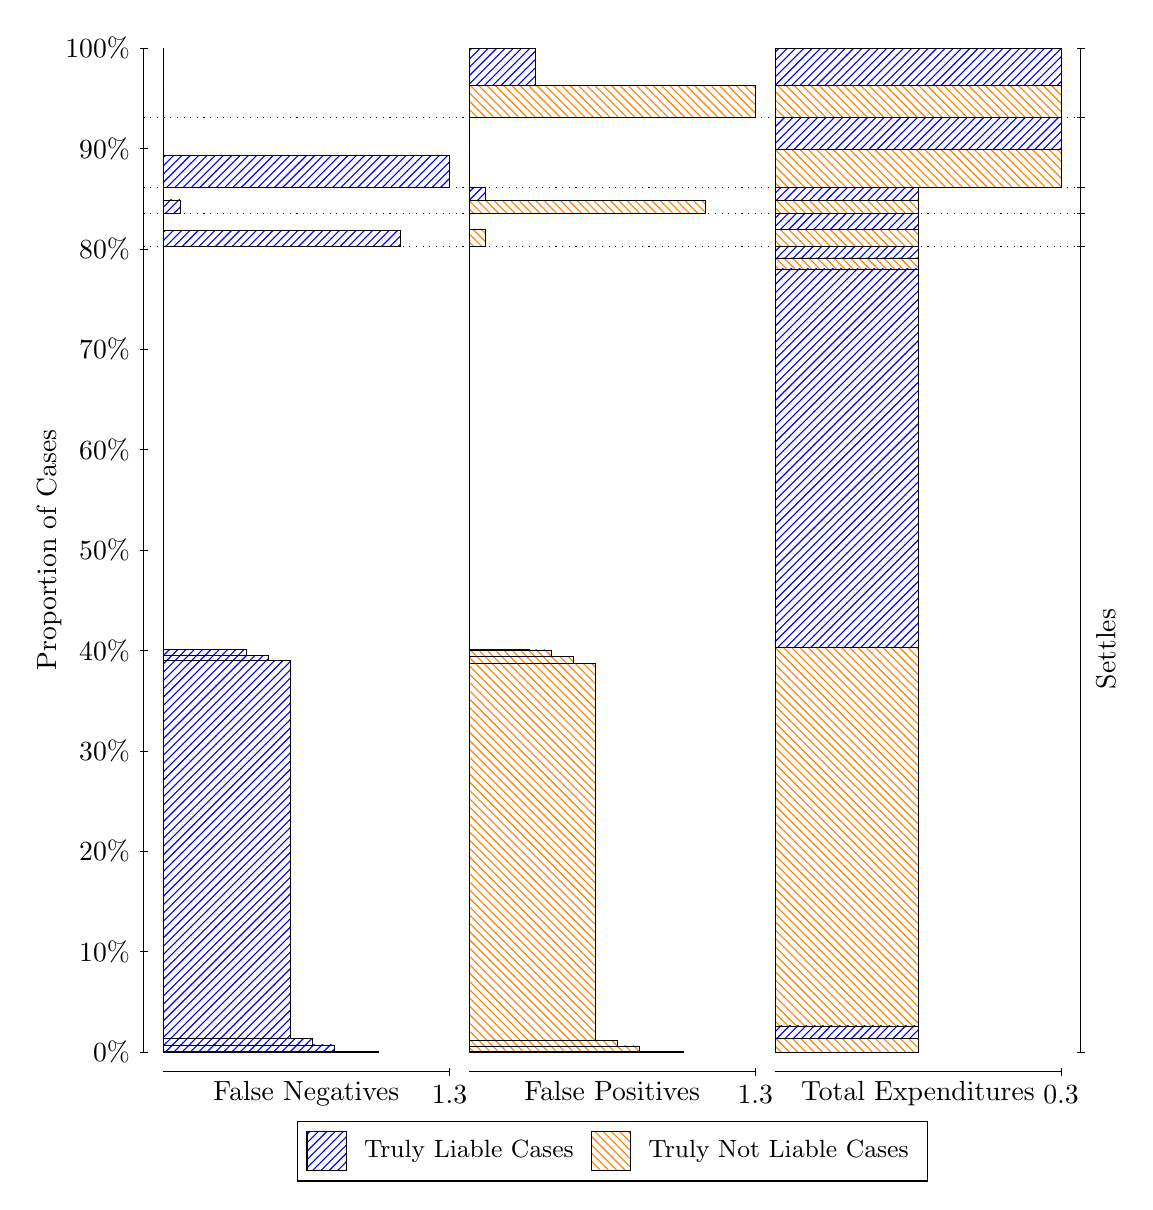
\begin{tikzpicture}
\draw[black, very thin] (1.5,1.75) -- (1.5,14.5);
\node[rotate=90, anchor=center] at (0.3, 8.125) {Proportion of Cases};
\draw[black, very thin] (1.45,1.75) -- (1.55,1.75);
\node[anchor=east] at (1.45, 1.75) {0\%};
\draw[black, very thin] (1.45,3.025) -- (1.55,3.025);
\node[anchor=east] at (1.45, 3.025) {10\%};
\draw[black, very thin] (1.45,4.3) -- (1.55,4.3);
\node[anchor=east] at (1.45, 4.3) {20\%};
\draw[black, very thin] (1.45,5.575) -- (1.55,5.575);
\node[anchor=east] at (1.45, 5.575) {30\%};
\draw[black, very thin] (1.45,6.85) -- (1.55,6.85);
\node[anchor=east] at (1.45, 6.85) {40\%};
\draw[black, very thin] (1.45,8.125) -- (1.55,8.125);
\node[anchor=east] at (1.45, 8.125) {50\%};
\draw[black, very thin] (1.45,9.4) -- (1.55,9.4);
\node[anchor=east] at (1.45, 9.4) {60\%};
\draw[black, very thin] (1.45,10.675) -- (1.55,10.675);
\node[anchor=east] at (1.45, 10.675) {70\%};
\draw[black, very thin] (1.45,11.95) -- (1.55,11.95);
\node[anchor=east] at (1.45, 11.95) {80\%};
\draw[black, very thin] (1.45,13.225) -- (1.55,13.225);
\node[anchor=east] at (1.45, 13.225) {90\%};
\draw[black, very thin] (1.45,14.5) -- (1.55,14.5);
\node[anchor=east] at (1.45, 14.5) {100\%};

\draw[black, very thin] (13.4,1.75) -- (13.4,14.5);
\draw[black, very thin] (13.35,1.75) -- (13.45,1.75);
\node[anchor=west] at (13.35, 1.75) {};
\draw[black, very thin] (13.35,11.985) -- (13.45,11.985);
\node[anchor=west] at (13.35, 11.985) {};
\draw[black, very thin] (13.35,12.398) -- (13.45,12.398);
\node[anchor=west] at (13.35, 12.398) {};
\draw[black, very thin] (13.35,12.733) -- (13.45,12.733);
\node[anchor=west] at (13.35, 12.733) {};
\draw[black, very thin] (13.35,13.617) -- (13.45,13.617);
\node[anchor=west] at (13.35, 13.617) {};
\draw[black, very thin] (13.35,14.5) -- (13.45,14.5);
\node[anchor=west] at (13.35, 14.5) {};

\draw[black, very thin, pattern color=blue, pattern=north east lines] (1.75,1.75) rectangle (4.475,1.7588);
\draw[black, very thin, pattern color=blue, pattern=north east lines] (1.75,1.7588) rectangle (4.1955,1.76);
\draw[black, very thin, pattern color=blue, pattern=north east lines] (1.75,1.76) rectangle (3.916,1.8403);
\draw[black, very thin, pattern color=blue, pattern=north east lines] (1.75,1.8403) rectangle (3.6365,1.9211);
\draw[black, very thin, pattern color=blue, pattern=north east lines] (1.75,1.9211) rectangle (3.3571,6.7187);
\draw[black, very thin, pattern color=blue, pattern=north east lines] (1.75,6.7187) rectangle (3.0776,6.7882);
\draw[black, very thin, pattern color=blue, pattern=north east lines] (1.75,6.7882) rectangle (2.7981,6.8595);
\draw[black, very thin, pattern color=blue, pattern=north east lines] (1.75,6.8595) rectangle (2.5186,6.8623);
\draw[black, very thin, pattern color=blue, pattern=north east lines] (1.75,6.8623) rectangle (2.2391,6.8676);
\draw[black, very thin, pattern color=orange, pattern=north west lines] (1.75,6.8676) rectangle (1.75,11.985);
\draw[black, very thin, pattern color=blue, pattern=north east lines] (1.75,11.985) rectangle (4.7545,12.187);
\draw[black, very thin, pattern color=orange, pattern=north west lines] (1.75,12.187) rectangle (1.75,12.398);
\draw[black, very thin, pattern color=blue, pattern=north east lines] (1.75,12.398) rectangle (1.9596,12.57);
\draw[black, very thin, pattern color=orange, pattern=north west lines] (1.75,12.57) rectangle (1.75,12.733);
\draw[black, very thin, pattern color=blue, pattern=north east lines] (1.75,12.733) rectangle (5.3833,13.139);
\draw[black, very thin, pattern color=orange, pattern=north west lines] (1.75,13.139) rectangle (1.75,13.617);
\draw[black, very thin, pattern color=orange, pattern=north west lines] (1.75,13.617) rectangle (1.75,14.022);
\draw[black, very thin, pattern color=blue, pattern=north east lines] (1.75,14.022) rectangle (1.75,14.5);
\draw[black, very thin, pattern color=orange, pattern=north west lines] (5.6333,1.75) rectangle (8.3583,1.755);
\draw[black, very thin, pattern color=orange, pattern=north west lines] (5.6333,1.755) rectangle (8.0788,1.7578);
\draw[black, very thin, pattern color=orange, pattern=north west lines] (5.6333,1.7578) rectangle (7.7994,1.826);
\draw[black, very thin, pattern color=orange, pattern=north west lines] (5.6333,1.826) rectangle (7.5199,1.8926);
\draw[black, very thin, pattern color=orange, pattern=north west lines] (5.6333,1.8926) rectangle (7.2404,6.6888);
\draw[black, very thin, pattern color=orange, pattern=north west lines] (5.6333,6.6888) rectangle (6.9609,6.7721);
\draw[black, very thin, pattern color=orange, pattern=north west lines] (5.6333,6.7721) rectangle (6.9609,6.7733);
\draw[black, very thin, pattern color=orange, pattern=north west lines] (5.6333,6.7733) rectangle (6.6814,6.8571);
\draw[black, very thin, pattern color=orange, pattern=north west lines] (5.6333,6.8571) rectangle (6.4019,6.8583);
\draw[black, very thin, pattern color=orange, pattern=north west lines] (5.6333,6.8583) rectangle (6.1224,6.8674);
\draw[black, very thin, pattern color=blue, pattern=north east lines] (5.6333,6.8674) rectangle (5.6333,11.985);
\draw[black, very thin, pattern color=orange, pattern=north west lines] (5.6333,11.985) rectangle (5.8429,12.196);
\draw[black, very thin, pattern color=blue, pattern=north east lines] (5.6333,12.196) rectangle (5.6333,12.398);
\draw[black, very thin, pattern color=orange, pattern=north west lines] (5.6333,12.398) rectangle (8.6378,12.562);
\draw[black, very thin, pattern color=blue, pattern=north east lines] (5.6333,12.562) rectangle (5.8429,12.733);
\draw[black, very thin, pattern color=orange, pattern=north west lines] (5.6333,12.733) rectangle (5.6333,13.211);
\draw[black, very thin, pattern color=blue, pattern=north east lines] (5.6333,13.211) rectangle (5.6333,13.617);
\draw[black, very thin, pattern color=orange, pattern=north west lines] (5.6333,13.617) rectangle (9.2667,14.022);
\draw[black, very thin, pattern color=blue, pattern=north east lines] (5.6333,14.022) rectangle (6.4718,14.5);
\draw[black, very thin, pattern color=orange, pattern=north west lines] (9.5167,1.75) rectangle (11.333,1.9195);
\draw[black, very thin, pattern color=blue, pattern=north east lines] (9.5167,1.9195) rectangle (11.333,2.0818);
\draw[black, very thin, pattern color=orange, pattern=north west lines] (9.5167,2.0818) rectangle (11.333,6.8871);
\draw[black, very thin, pattern color=blue, pattern=north east lines] (9.5167,6.8871) rectangle (11.333,11.694);
\draw[black, very thin, pattern color=orange, pattern=north west lines] (9.5167,11.694) rectangle (11.333,11.836);
\draw[black, very thin, pattern color=blue, pattern=north east lines] (9.5167,11.836) rectangle (11.333,11.985);
\draw[black, very thin, pattern color=orange, pattern=north west lines] (9.5167,11.985) rectangle (11.333,12.196);
\draw[black, very thin, pattern color=blue, pattern=north east lines] (9.5167,12.196) rectangle (11.333,12.398);
\draw[black, very thin, pattern color=orange, pattern=north west lines] (9.5167,12.398) rectangle (11.333,12.562);
\draw[black, very thin, pattern color=blue, pattern=north east lines] (9.5167,12.562) rectangle (11.333,12.733);
\draw[black, very thin, pattern color=orange, pattern=north west lines] (9.5167,12.733) rectangle (13.15,13.211);
\draw[black, very thin, pattern color=blue, pattern=north east lines] (9.5167,13.211) rectangle (13.15,13.617);
\draw[black, very thin, pattern color=orange, pattern=north west lines] (9.5167,13.617) rectangle (13.15,14.022);
\draw[black, very thin, pattern color=blue, pattern=north east lines] (9.5167,14.022) rectangle (13.15,14.5);
\draw[black, dotted] (1.5,11.985) -- (13.4,11.985);
\draw[black, dotted] (1.5,12.398) -- (13.4,12.398);
\draw[black, dotted] (1.5,12.733) -- (13.4,12.733);
\draw[black, dotted] (1.5,13.617) -- (13.4,13.617);
\draw[black, very thin] (1.75,1.5) -- (5.3833,1.5);
\node[anchor=north] at (3.5667, 1.5) {False Negatives};
\draw[black, very thin] (5.3833,1.45) -- (5.3833,1.55);
\node[anchor=north] at (5.3833, 1.45) {1.3};

\draw[black, very thin] (5.6333,1.5) -- (9.2667,1.5);
\node[anchor=north] at (7.45, 1.5) {False Positives};
\draw[black, very thin] (9.2667,1.45) -- (9.2667,1.55);
\node[anchor=north] at (9.2667, 1.45) {1.3};

\draw[black, very thin] (9.5167,1.5) -- (13.15,1.5);
\node[anchor=north] at (11.333, 1.5) {Total Expenditures};
\draw[black, very thin] (13.15,1.45) -- (13.15,1.55);
\node[anchor=north] at (13.15, 1.45) {0.3};

\node[black, centered, rotate=90] at (13.72, 6.8675) {Settles};





\draw (7.449999999999999,1.5) node[draw=none] (baseCoordinate) {};
\begin{scope}[align=center]
        \matrix[scale=0.5, draw=black, below=0.5cm of baseCoordinate, nodes={draw}, column sep=0.1cm]{
            \node[rectangle, draw, minimum width=0.5cm, minimum height=0.5cm, pattern=north east lines, pattern color=blue] {}; &
            \node[draw=none, font=\small] (B) {Truly Liable Cases}; &
            \node[rectangle, draw, minimum width=0.5cm, minimum height=0.5cm, pattern=north west lines, pattern color=orange] {}; &
            \node[draw=none, font=\small] (B) {Truly Not Liable Cases}; \\
            };
\end{scope}

\end{tikzpicture}
\end{document}